\documentclass[a4paper,12pt]{article}
% Use the options 'crop' to show crop marks, and
% 'doublespaced' for double line spacing.
% e.g. \documentclass[crop,doublespaced]{cupjournal}


%calling packages
\usepackage[english]{babel}
\usepackage[utf8]{inputenc}
\usepackage{amsmath}
\usepackage{graphicx}
\usepackage[left=1in,right=1in,top=1in,bottom=1in]{geometry}
\usepackage{setspace}
\usepackage[round]{natbib}
\usepackage{epstopdf}
\usepackage{soul}
\usepackage{lmodern}
\usepackage{caption}
\usepackage{hyperref}
\usepackage{subcaption}
\usepackage{rotating}
%\usepackage{etoc}


\usepackage{xr}
%\externaldocument{"appendix"}


\usepackage{longtable}
\usepackage{amssymb}
\usepackage{fancyhdr}
\usepackage{array}
\usepackage{lscape} % for landscape formatting of pages
\newcolumntype{P}[1]{>{\centering\arraybackslash}p{#1}}
%fonts
\usepackage{times}
%\setcounter{secnumdepth}{0}
%chanfing font of table headers
\captionsetup[figure]{labelfont=bf}
\captionsetup[table]{labelfont=bf}

%path to where figures are located
\graphicspath{ {images/} }

%for notes in table captions 
\newcommand\fnote[1]{\captionsetup{font=small}\caption*{#1}}

%changing header
\pagestyle{fancy}
\fancyhf{}
\rhead{\thepage}
\renewcommand{\headrulewidth}{0pt}
\renewcommand{\footrulewidth}{0pt}
\renewcommand*\footnoterule{}
\let\svfootnoterule\footnoterule
\renewcommand\footnoterule{\vspace{0.2in}\svfootnoterule}
\renewcommand*{\thefootnote}{\fnsymbol{footnote}}
%set spacing

\renewcommand{\sfdefault}{phv}

\doublespacing
\usepackage{titlesec}

\titleformat*{\section}{\Large\sffamily}
\titleformat*{\subsection}{\large\sffamily}
\titlespacing*\section{0pt}{24pt plus 4pt minus 2pt}{4pt plus 2pt minus 2pt}
\titlespacing*\subsection{0pt}{20pt plus 4pt minus 2pt}{4pt plus 2pt minus 2pt}


%changing title settings
\makeatletter
\renewcommand{\maketitle}{
	\begin{flushleft}
		
		\onehalfspacing
		
		\@title
		
		\lineskip .5em
		\normalfont{\normalsize{\@author}}
\end{flushleft}}
\makeatother


\newcommand{\beginsupplement}{%
	\setcounter{table}{0}
	\renewcommand{\thetable}{S.\arabic{table}}%
	\setcounter{figure}{0}
	\renewcommand{\thefigure}{S.\arabic{figure}}%
}


%title
\title{\bigskip \bigskip \sffamily \LARGE{Can Citizens Set City Policy?} \\ \Large{ Evidence From A Decentralized Welfare State}}

%author
\author{\bigskip Benjamin Carl Egerod\footnote[2]{Graduate Student, Department of Political Science, University of Copenhagen, e-mail: \texttt{benjamin.carl.egerod@ifs.ku.dk}.} \qquad Martin Vinæs Larsen\footnote[3]{Assistant Professor, Department of Political Science, Aarhus University, e-mail: \texttt{mvl@ps.au.dk}.}} 



\begin{document}

	
	\begin{footnotesize} \noindent \today. \end{footnotesize} %date
	
	\vspace{0.7in}
	
	\maketitle
	
	\bigskip
	
	\begin{quotation} %abstract

		\small \noindent \emph{Abstract:} Municipal governments supposedly empower citizens, giving them the ability to shape the political organization of their local community. In spite of this, we know little about whether municipal governments are in fact responsive to the policy views of municipal electorates. In this study, we look at whether the policy implemented by local politicians actually respond to changes in the public mood. To do this, we compile a unique and comprehensive dataset of local fiscal policy, which we use to construct municipal-level estimates of fiscal policy conservatism. This detailed policy data is then linked to an indicator of local ideological sentiment. We find strong evidence for dynamic responsiveness: when preferences in a municipality changes public policy responds.
	\end{quotation}



	
	\thispagestyle{empty} %removing page number from page one
	
	
\clearpage


\noindent In most developed countries municipal governments are an essential part of representative government \citep{trounstine2009all,kersting2013reforming}. They are responsible for a large part of public spending.  They are able to levy taxes on income and property. And while they are subordinate to central governments, oversight is always limited in formal or informal ways \citep{oecd2016subnational}. In this way, municipalities play a central part in the quintessential political act of deciding who gets what, when and how. From the standpoint of democratic representation it is thus interesting to ask: is it the citizens in the municipality that set policy or is it set for them by extraneous forces?

There is good reason to be skeptical of municipal governments' democratic potential. For one,  several forces limit municipal governments capacity to respond to public concerns. Central governments put constraints on local government decision-making \citep{peterson1981city}. Competition with other adjacent municipalities restrain policy-making \citep{salmon2006horizontal,tiebout1956pure}. Further, even if municipalities can set policy, voters might not be able to hold local officials accountable\citep[e.g.,][]{sances2017attribution} As such, local elections are often considered second-order by voters \citep[e.g.,][]{marsh1998testing}. As a result, voters might have a hard time electing politicians who match their preferences in local elections. 



Recent empirical studies of municipal government, however, suggest that such concerns might not be warranted.  A number of studies have shown that voters tend to (re-)elect local politicians based on their actions in office \citep{arnold2012holding,burnett2017politics,boyne2009democracy} and that voters tend to vote for conservative (liberal)  mayors if they themselves hold conservative (liberal) policy views  \citep{sances2017ideology,boudreau2015lost,hopkins2017retrospective}. Furthermore, a number of studies have found that it matters for city policy whether a conservative or a liberal party controls the mayoralty and/or the city council \citep{fiva2016power,folke2014shades,blom2006parties,de2016mayoral}. 

While these studies provide \textit{indirect} evidence that municipalities are responsive, there are only a few studies that examine municipal responsiveness more directly. Most notably, Tausanovitch and Warshaw's recent influential study  was the first comprehensive examination of the responsiveness of city policy \citep{tausanovitch2014representation}. In this study, the authors uses Multilevel Regression with Poststratification (MRP) to estimate the policy preferences of citizens in a cross section of US cities. They find a strong and robust correlation between these preferences and city policy \citep[see also][]{hajnal2010or,palus2010responsiveness}. Since then, two other studies have directly examined municipal responsiveness. The first of these are \cite{einstein2016pushing}. Here, the authors also identify a strong correlation between citizen preferences, measured as support for the Democratic party at presidential elections,  and city policy. Apart from replicating the findings from \citeauthor{tausanovitch2014representation}, \citeauthor{einstein2016pushing} are also able to identify the use of intergovernmental grants as a key mechanism underlying responsiveness. They also offer a stronger identification strategy by examining responsiveness in a panel of cities from two US states using a lagged dependent variable approach. In an unpublished study, \cite{sances2017voters} expands on existing work using a panel of 3,000 US counties spanning 50 years. Linking changes in Democratic vote share to county-level policy, \citeauthor{sances2017voters} finds that as counties grow more Democratic they tend to spend more and to collect more own-source revenues.





All in all, research in the area of municipal responsiveness has made impressive progress in the past few years, however, the existing evidence remains limited in different important ways. First, city policy is usually measured using either few indicators \citep{sances2017voters,einstein2016pushing} or at a single point in time \citep{tausanovitch2014representation}. Relatedly, few have looked at whether changes in preferences from election to election produce change in future city policy. In fact, most previous analysis is either cross-sectional or looks at concurrent changes in policy and preferences. This is in part a methodological problem, as the risk of reverse causation looms large when we measure policy and preferences at the same time. However, the static analysis which permeates most of the existing literature also puts limits on what theoretical inferences we can make: in particular, it is hard to know whether municipalities are dynamically responsive \citep{stimson1995dynamic}. Finally, the existing literature is almost exclusively based in the US, which naturally raises concerns about generalisability.


In this study, we address these limitations related to context, design and data by studying responsiveness in Danish municipalities. In particular, we develop an annual measure of municipal policy conservatism based on 14 fiscal policy indicators (1978-2006). A measure which is much more comprehensive in terms of its granularity, and the time period covered, than the city policy measures used in previous studies. Similar to previous studies, we use net support for conservative (right-wing) parties as a proxy for policy views, but unlike previous studies, which had to rely on electoral support measured at national or regional elections, we are able to look at electoral support at \textit{local} elections dating back to 1970. 

Using this comprehensive dataset, we link past changes in preferences to future changes in policy to avoid concerns about reverse causality. We find that changes in the policy preferences of citizens have substantial effects on city policy. We also show that there is no evidence of reverse causality---i.e., past changes in policy do not predict future changes in preferences--- and that our findings are not driven by  fiscal stress. Our findings thus suggest that, at least to some extent, citizens do set city policy.


\section*{Empirical Strategy}

 We examine municipal responsiveness in Denmark. Denmark is a decentralized welfare state where municipalities can affect their local revenue and set a yearly budget.  Municipal tasks and services include the core welfare services of the Danish welfare state and municipal spending amounts to 35 percent of GDP, which is more than half of all public spending. We focus on Denmark, as this allows us to track the relationship between citizen preferences and city policy in a dynamic way. We are able to get a detailed measure of city policy for all years between 1978 and 2005 for all 271 Danish municipalities. This is unique as previous studies have had to rely on policy measured at one point in time \citep{tausanovitch2014representation,palus2010responsiveness} or measured with substantial intervals\citep{sances2017voters,einstein2016pushing,hajnal2010or}. Further, we can link this to preferences as expressed for right and left wing parties in municipal elections in the same period. As such, unlike most previous research, we do not have to infer that voters preferences for progressive policies are the same at the national and the local level \citep[for an exception, see][]{tausanovitch2014representation}. Finally, by examining Danish municipalities we are able to move away from the US political context, which has been the sole focus of previous studies. 
 
Danish municipalities are radically different from US counties and cities. They are small (average size 16,000), organized in general rather than special purpose governments \citep{berry2009imperfect}, with a multi party, PR system where turnout is relatively high.\footnote{See Appendix \ref{context} for more details on the Danish system} It is thus not clear whether Denmark is an easy or hard case for responsiveness, as some factors--such as the small size of the municipalities--seem to make responsiveness less likely than in the US, whereas others--such as the general purpose organization of local government--seem to make responsiveness more likely. As such, the Danish case can not be seen as especially typical or atypical. Instead, what makes the Danish case interesting is the high quality data on municipal policy and municipal policy preferences which are available, and the fact that it is a very different setting from the ones previously examined.


\subsection*{An Annual Measure of Municipal Fiscal Policy Conservatism}

To measure fiscal policy conservatism in Danish municipalities we rely on 14 different indicators relating to either tax policy (3 indicators), spending policy (2), organization of public service delivery (3), co-payment for public services (4) or the extent of public services (2). Variables measured in DKKs are adjusted for inflation. While  spending and tax variables are commonly used in the literature, we are the first to include other types of variables in a panel set-up. An overview of the policy indicators are presented in Appendix \ref{policy}

The included policies had to meet the following criteria: (1) The policy should be directly set by the city council.\footnote{It was included even if it was set in collaboration between the city council and some other (set of) actor(s).} (2) It had to be a policy and not the outcome of a policy (i.e., we did not include unemployment). (3) Data on the policy had to be available for at least five years between 1978 and 2016. All policy information was retrieved from Statistics Denmark or the Danish Ministry for Economic Affairs and the Interior.

We combine these 14 indicators into an index of fiscal policy conservatism. Inspired by \cite{caughey2016dynamics} analysis of US states, we use a Bayesian latent variable technique to estimate municipal fiscal conservatism as a latent trait driving municipal policies. 

This method is in many ways similar to frequentist factor analysis. However, a major advantage to using Bayesian techniques when making inferences about the latent trait is that the simulations will impute missing data during the estimation, which allows us to include items with different numbers of observations in the model -- the variables with missing observations will simply supply less information to the estimation. Finally, the estimation is simulation based, which allows us to directly estimate uncertainty around all model parameters.

Using this technique is particularly important in this case, because data on most indicators is only available after 1993. However, because we use this measurement method they still shape our estimates of municipal fiscal policy conservatism across the entire period. Details about the measurement model can be found in Appendix \ref{estimation}. 

Even so, variables with missing values supply less information to our measure in periods, where we have no data on them. Accordingly, our measure of fiscal policy conservatism for the period 1978-1992 primarily relies on the measures of income tax, property tax and spending pr. capita. To make sure that our results are not driven by the inclusion of different items at various points in time, we do all analyses below using only these three variables (reduced measure) as well as with all indicators (full measure).

Both our reduced and our full measure is standardized to have mean zero and a standard deviation of one. In Appendix \ref{descriptives}, we show how municipal policy conservatism varies across time and place in Denmark.



\subsection*{Municipal Policy Preferences}

In order to find out whether municipal fiscal policy conservatism responds to the preferences of the electorate, we need to develop a measure of local policy preferences. In line with previous work on municipal responsiveness \cite[e.g.,][]{sances2017ideology,einstein2016pushing}, we measure local policy preferences indirectly by examining the net difference in electoral support for right-wing and left-wing parties in the municipality, inferring that municipal electorates which prefer conservative parties also prefer conservative fiscal policies. In particular, we look at the difference between support for the major center-right parties as well as the right wing populist parties (Venstre, Det Konservative Folkeparti, Fremskridstpartiet and Dansk Folkeparti) and the major center-left parties as well as the socialist parties (Socialdemokratiet, Radikale Venstre, Socialistisk Folkeparti, Venstresocialisterne, and Enhedslisten) at all municipal elections in the period under study. This gives us an estimate of local policy preferences in the years 1974, 1978, 1981, 1985, 1989, 1993, 1997 and 2001.

 Unlike previous studies, which have had to rely on support for conservative vis-a-vis liberal parties at national or regional elections \citep[e.g.,]{hajnal2010or,einstein2016pushing}, we are able to look at support at municipal elections. This is potentially important, as citizens might differ in their policy views across domains \cite[for an argument along these lines, see]{abrams2012big}.  Why might there be a divergence between the electorate's preferences at a local and at a national election?  For one, the electorate at municipal elections might be differently composed than electorates in national elections, as different types of people participate in different types of elections \citep{ansolabehere2015beyond,hansen2017social}. Beyond this, there might be voters who wants more liberal fiscal policies locally and more conservative policies nationally. In Appendix  \ref{validation} we show that there is added value in using municipal rather than national election returns. In particular,we find that in a concurrent municipal and national election net support for is far from perfectly correlated (Pearsons R=0.56).
 
 It might have been preferable to have actual estimates of citizens preferences over policy using an MRP approach \citep[similar to the measure used by][]{tausanovitch2014representation}. Doing so is not feasible, as survey data is too sparse, especially for the earlier part of the period we study. Instead, we do a validation of our measure in Appendix \ref{validation}, where we show that there is a strong correlation between net support for conservative parties at municipal elections and citizens answers on ideology questions, using some recent survey data.


\section*{Identifying Dynamic Responsiveness in Cities}
Figure \ref{fig:scatter} shows that the past changes in support for right-wing parties are related to future changes in fiscal concervatism (full measure), suggesting that  policy adjusts dynamically to changes in preferences. This is striking, as we have minimized concerns related to reverse causality, since  future changes in policy cannot affect past changes in preferences.

\begin{figure}[h]
	\centering
	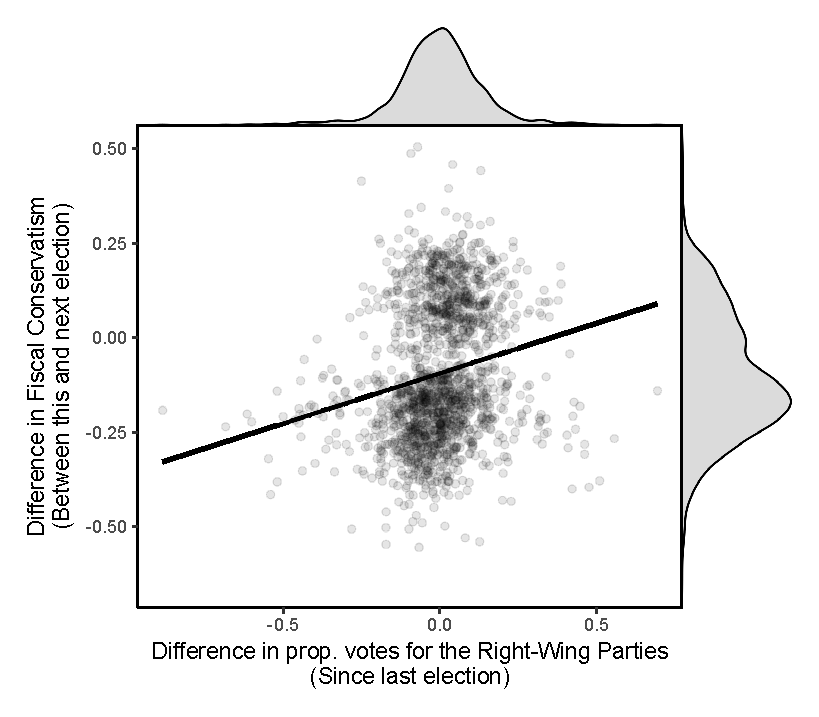
\includegraphics[scale = 1.2]{fd_plot.eps}
	\caption{Do Changes in Voter Mood Correlate with Changes in Policy? Fitted line is a loess smoother, densities show the marginal distributions of both variables.}
	\label{fig:scatter}
\end{figure}

We model this relationship formally in four different ways. A (1) fixed effects model (municipality and year) regressing net support for conservative parties at a given election on municipal fiscal conservatism four years later (corresponding to an election period), (2) a model allowing for municipalities to be on different time trends (3) a pooled model which excludes the time and year fixed effects, and (4) a first difference model that directly models the data from Figure \ref{fig:scatter}. All models include a control for population size (logged), but the results do not depend on this covariate.

Figure \ref{fig:FourYearLead} plots the key estimate (i.e., the effect of changes in local policy preferences) from these models. The  left panel uses the full measure of fiscal conservatism as the dependent variable whereas the right panel uses our reduced measure. Across all four models we find a statistically significant and positive effect. Furthermore, we obtain the same results using either measure of fiscal conservatism (differences in the unstandardized coefficients are driven by a larger standard deviation in the reduced measure).

%This means that if net support for right-wing parties increases with 10 percentage points, then policy becomes XX more conservative. 

In our preferred fixed effects model, we estimate the effect to be roughly .12. If we only look at within municipality variation in policy conservatism, then this corresponds to 25 pct. of a standard deviation.  This is a substantive association. With an effect of this magnitude, moving the voters from the socialdemocratic stronghold Albertslund to the highly conservative Gentofte would transform the fiscal policy in Gentofte to roughly that of Slagelse. This would move Gentofte down by more than 40 positions (out of 273 municipalities) in our ranking of fiscal conservatism.

The identifying assumption in the twoway fixed effects model, is that trends in the dependent variable (policy) are independent of selection into the independent variable (preferences). If municipalities that experience changes in support for right-wing parties already were following different trends in policy this could bias our results. We relax the assumption by leveraging the Danish three-tier administrative setup, where municipalities are nested within regions. We interact the time fixed effects with a series of regional dummies as well as population size. This allows municipalities to be on separate time trends depending on both region (semi-parametrically) and population size (log-linearly). It also allows shocks to have heterogeneous effects depending on these factors. The changes to the estimates are diminutive.

Importantly, this strategy should also deal with the confounding effect of the socio-demographic make-up of the municipalities. To make sure that there is no remaining bias due to these factors, we include data on education, unemployment rate and the number of non-western immigrants in the municipality. Since these variables are only available after 1993, and there is a heavy trend in municipal policy, including them would bias our results by censoring the dependent variable. Instead, we follow \citep{pei2018poorly} and regress electoral support for right-wing parties on our three socio-demographic predictors. As we show in Appendix \ref{balance}, the correlations are very small and statistically insignificant. This suggests that these important socio-demographic factors cannot be driving our results. The null-correlation with unemployment is especially noteworthy, as it is a strong indicator of whether the municipality is hit particularly hard by a temporary economic shock, which might drive both preferences and policy.

In Appendix \ref{mechanism}, we examine whether municipal responsiveness is driven by selection. We do so in two ways: (1) by controlling for the mayoral party, and (2) by allowing responsiveness to vary by the mayoral party. Our results are remarkable in that they indicate that the mood in the electorate impacts policy no matter which party controls the mayoralty.

To examine the temporal dynamics of responsiveness, figure \ref{fig:LongRun} reports the estimated effect of local voter preferences at time $t$ on municipal policy (A) in the long run, and (B) how the baseline effect has changed over time. In particular, in panel A, we plot the effect on policy at the previous election (as a placebo), contemporaneously, and, respectively one, four, eight, 16 and 20 years into the future. This reveals that, as expected, it takes some time for policy to respond. There is only a small effect one year after local policy preferences change and the largest effect is  after four years. After this the effect seems to have some staying power, and while it disappears after the second election, it is remarkable that a change in voter mood can persist as far into the future as eight years (corresponding to two elections).


\begin{figure}[h]
	\centering
	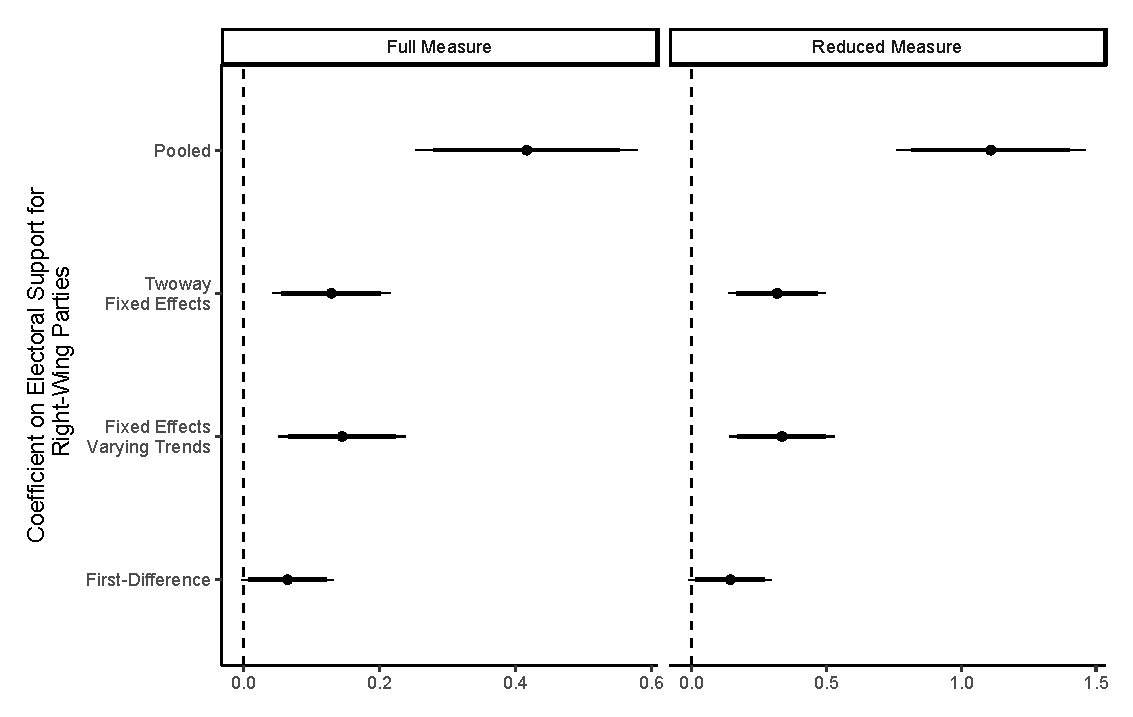
\includegraphics[scale = 0.8]{CoefPlot_18092018.eps}
	\caption{Effect of Electoral Support for Right-wing Parties with a 4-year Lead. Points are unstandardized OLS coefficients. Lines are 95 pct. (thin) and 90 pct. (thick) confidence intervals. Beck-Katz standard errors used in first-difference models, Arellano-White standard errors with clustering on municipality level used in the rest to correct for temporal autocorrelation.}
	\label{fig:FourYearLead}
\end{figure}


While we cannot test the identifying parallel trends assumption directly, we can see whether trends in the dependent are similar before municipalities "select into" different preferences. Importantly, if voters became \emph{more conservative} as a result of changes in policy \cite[cf.][]{lenz2013follow,slothuus2010can}, and this was what was driving our result, then we would expect pre-trends to be different. Figure \ref{fig:LongRun} shows that estimated effects of local policy preferences on policy conservatism at $t=-4$ are statistically insignificant and close to zero. Trends in social democratic and conservative municipalities are similar prior to the electorate's mood changes. After voter preferences evolve, however, trends in policy diverge.  This is notable, because it suggests that the key identifying assumption of our generalized difference in difference model hold. To further bolster this, in Appendix \ref{granger} we show that changes in municipal policy do not precede changes in electoral support for right-wing parties.

In Panel B we allow the effect of voter preferences on policy four years into the future to vary through time by including random slopes by year. The results show that municipal policy responsiveness is a relatively new thing -- prior to 1993 there was no correlation, and the baseline association seems to be driven by more recent years. This is an interesting exploratory finding, and future work could examine further the conditions under which we can expect city policy to be responsive.
 

\begin{figure}[h]
	\centering
	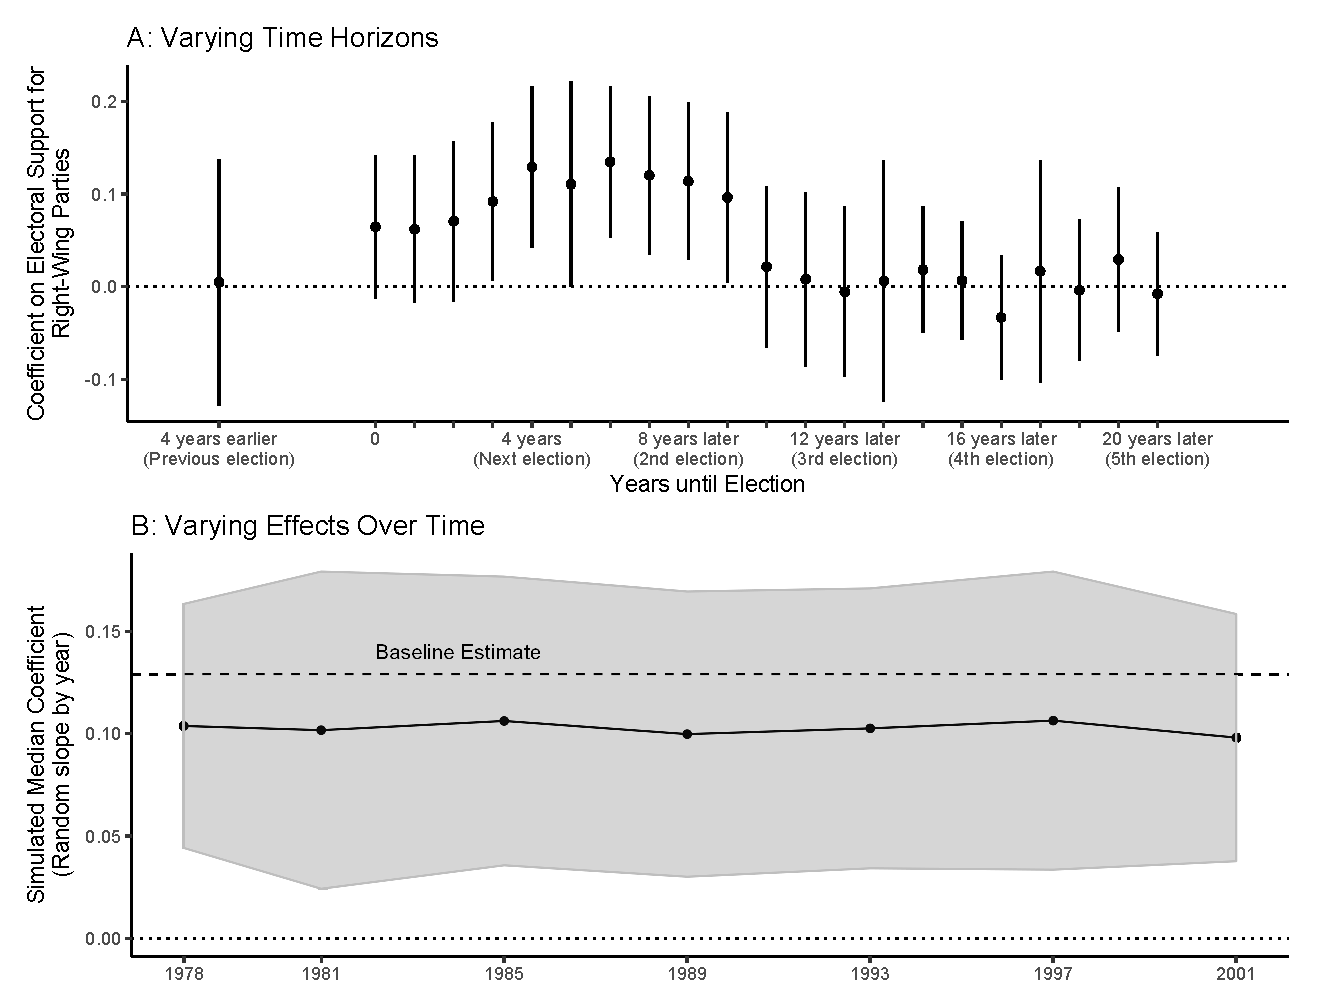
\includegraphics[scale = .6]{EffectsVsTime.eps}
	\caption{Effects of Local Policy Preferences Over Time. Black points represent the effect of net electoral support for conservative parties with different leads. Black lines are 95 pct. confidence intervals based on Arellano-White robust standard errors with clustering at the municipal level.}
	\label{fig:LongRun}
\end{figure}




\section*{Discussion \& Conclusion}



\onehalfspacing
%\bibliographystyle{apa}
%\bibliography{bibtex/library}

\clearpage

\renewcommand{\thesubsection}{\Alph{subsection}}
\renewcommand{\thetable}{\Alph{subsection}\arabic{table}}
\renewcommand{\thefigure}{\Alph{subsection}\arabic{figure}}


\end{document}

